\section{系统开发成果}

对基于Arduino的分布式温度控制系统已完成基本设计与开发,通过测试并于 2021 年 5 月运行在西安石油大学校内,校内网网址:\underline{http://arduino.deconf.xyz/}。将在机房自动化,校园环境智能化方面推进智能化校园建设。

\subsection{预期目标}

整体来说,本次系统设计和开发基本达成预期目标。

1. 提供了WEB页面可视化的管理和配置功能。可配置用户信息,节点信息等。

2. 关键信息的统计展示功能。完成了节点的温度、湿度、烟雾等信息的展示功能

3. 温度控制功能方面,通过Arduino传感器采集到的温度,在设定的阈值的控制下,通过红外发射模块,控制空调的温度。

3. 告警方面,在烟雾的值超过阈值之后,可以根据用户信息的电子邮箱发送对应的的告警信息。

\subsection{分布式节点管理控制系统}

依照前面的需求分析,系统设计等工作,确立了本系统采用C/S模型,来进行对各个节点的数据管控。按照前图\ref{fig:4-1}所示,进行S端的开发成果如下:

\subsubsection{用户模块}
按照模块化设计思想,实现用户模块如下所示。WEB端具有用户登录,用户注册,用户管理等功能。
用户登录具有用户鉴权,用户密码鉴别的能力,确保正确用户登录。用户注册可以使该系统支持多用户,且每个用户拥有属于自己的个人信息,以及关联的卡片信息等。用户管理方便管理员对多用户的修改,增加,删除等。用户的信息写入在后端存储的MySQL数据库中。在前端显示上做到了简洁大方以及美观。

\begin{figure}[htbp]
	\centering
	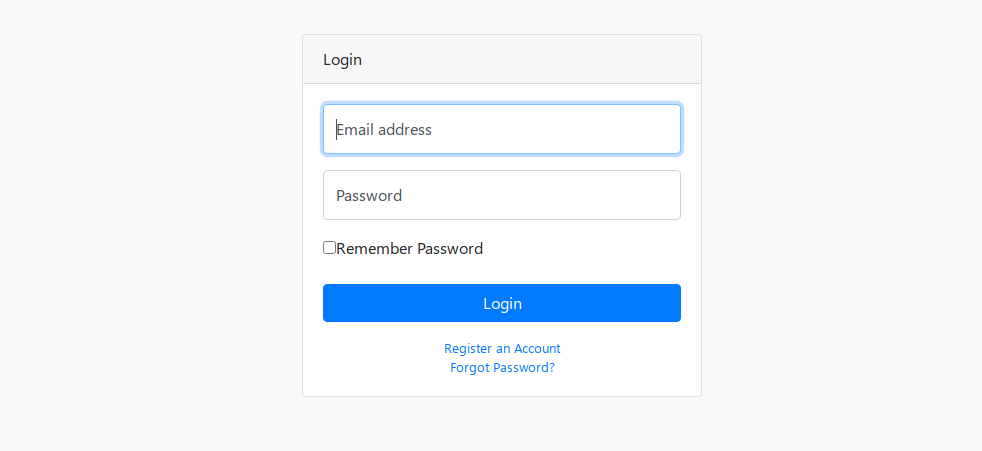
\includegraphics[width=0.85\linewidth]{figure/5-1}
	\caption{用户登录页面}
\end{figure}
\begin{figure}[H]
	\centering
	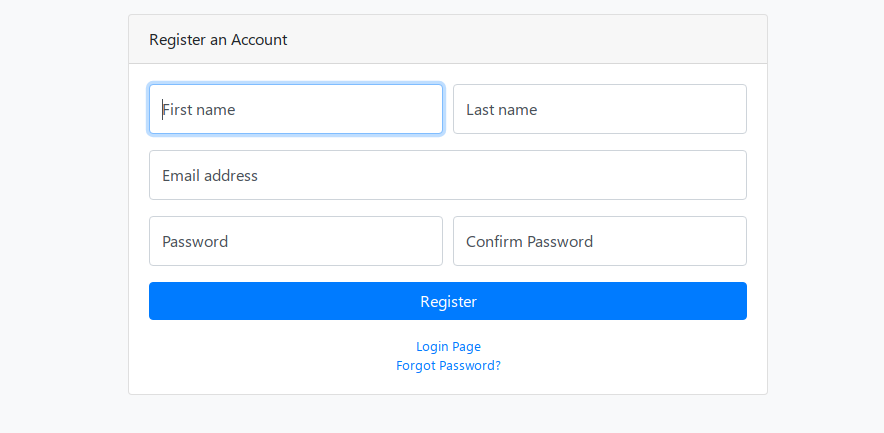
\includegraphics[width=0.85\linewidth]{figure/5-2}
	\caption{用户注册页面}
\end{figure}
\begin{figure}[H]
	\centering
	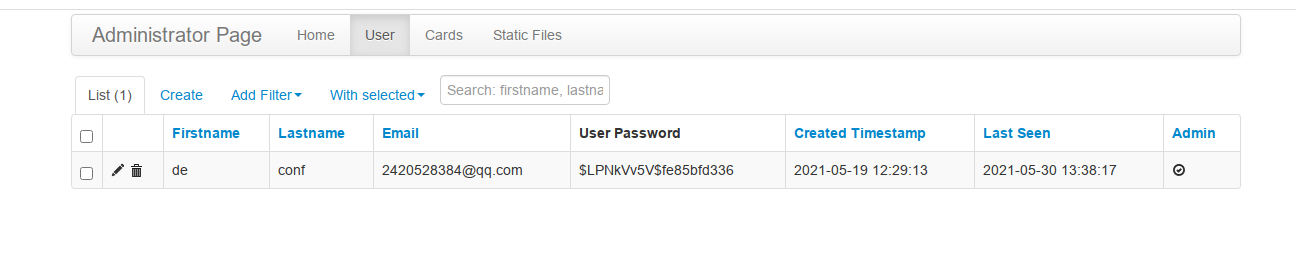
\includegraphics[width=0.85\linewidth]{figure/5-3}
	\caption{用户管理页面}
\end{figure}
\subsubsection{信息展示模块}
信息展示可以图形的方式直观的展示出节点的直观信息。方便直观的查看节点的环境参数,如当前的温度,湿度,烟雾等关键的环境信息,便于运维人员对于机房环境的监测。
\begin{figure}[H]
	\centering
	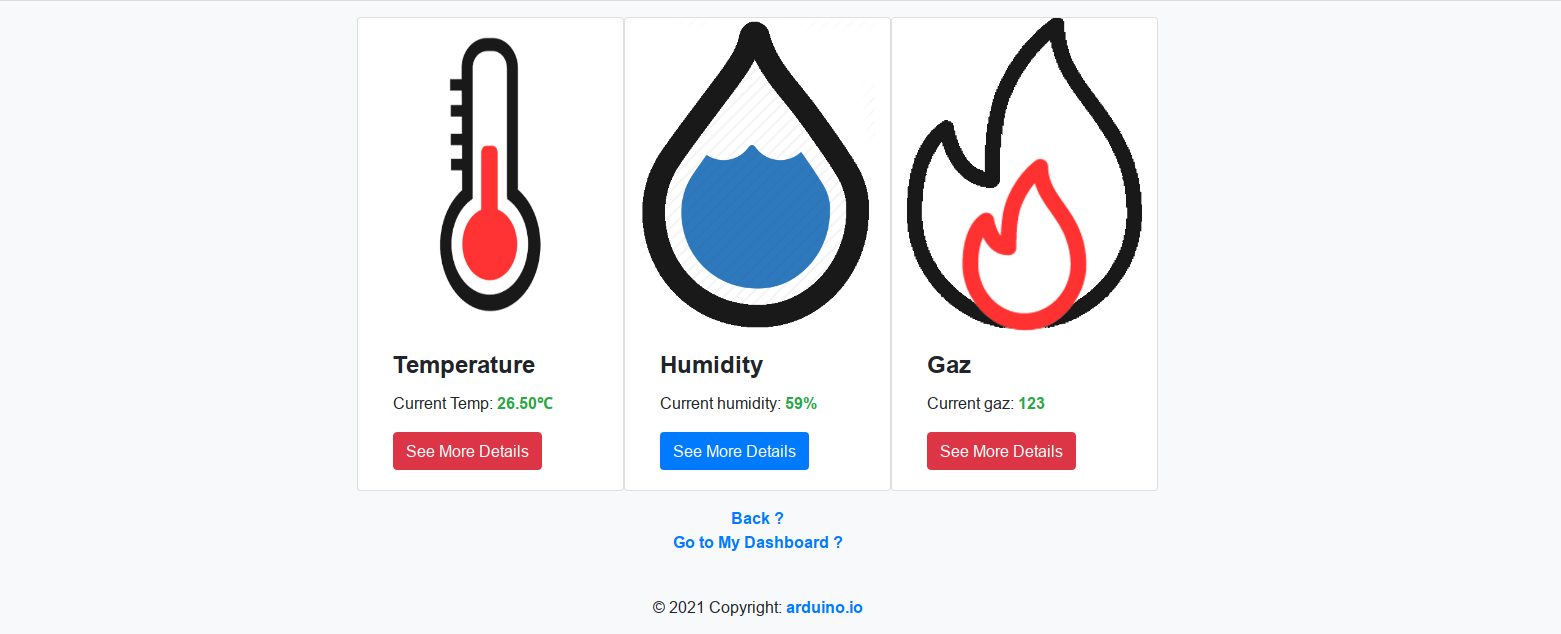
\includegraphics[width=0.85\linewidth]{figure/card_data}
	\caption{节点信息展示}
\end{figure}
\begin{figure}[H]
	\centering
	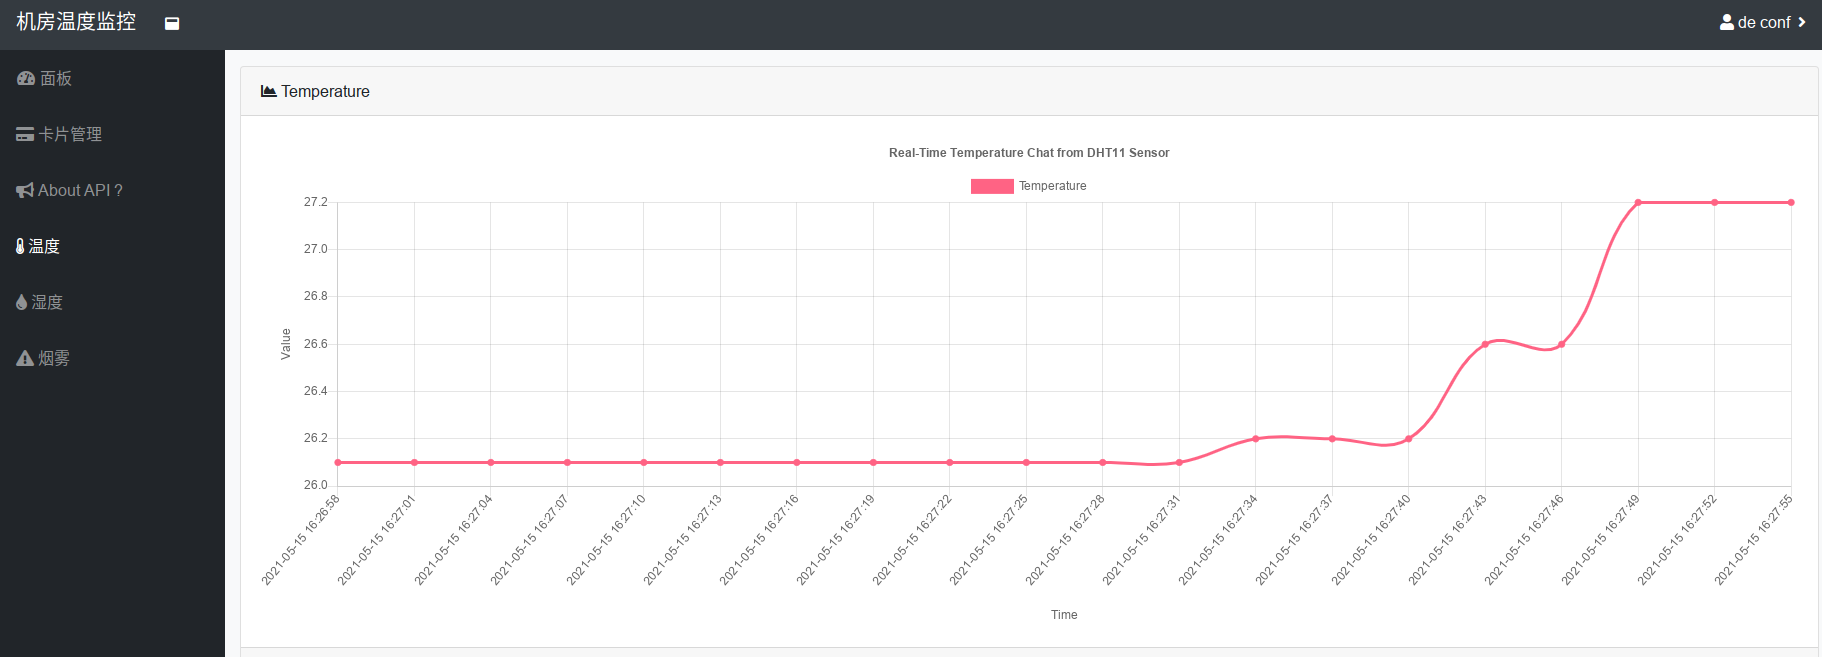
\includegraphics[width=0.85\linewidth]{figure/DHT11}
	\caption{温度显示模块}
\end{figure}
\begin{figure}[H]
	\centering
	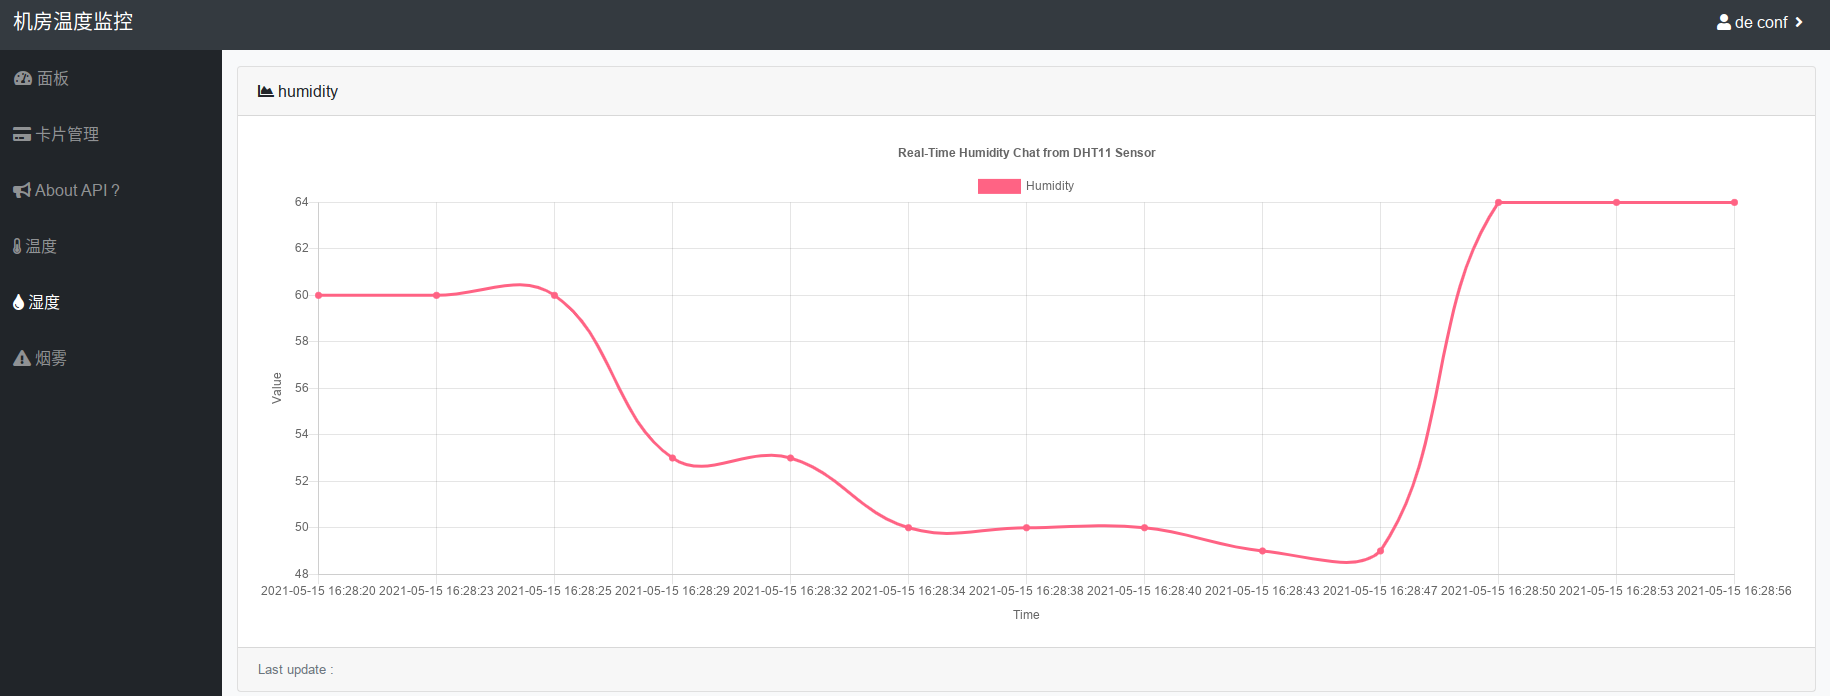
\includegraphics[width=0.85\linewidth]{figure/Humidity}
	\caption{湿度显示模块}
\end{figure}
\begin{figure}[H]
	\centering
	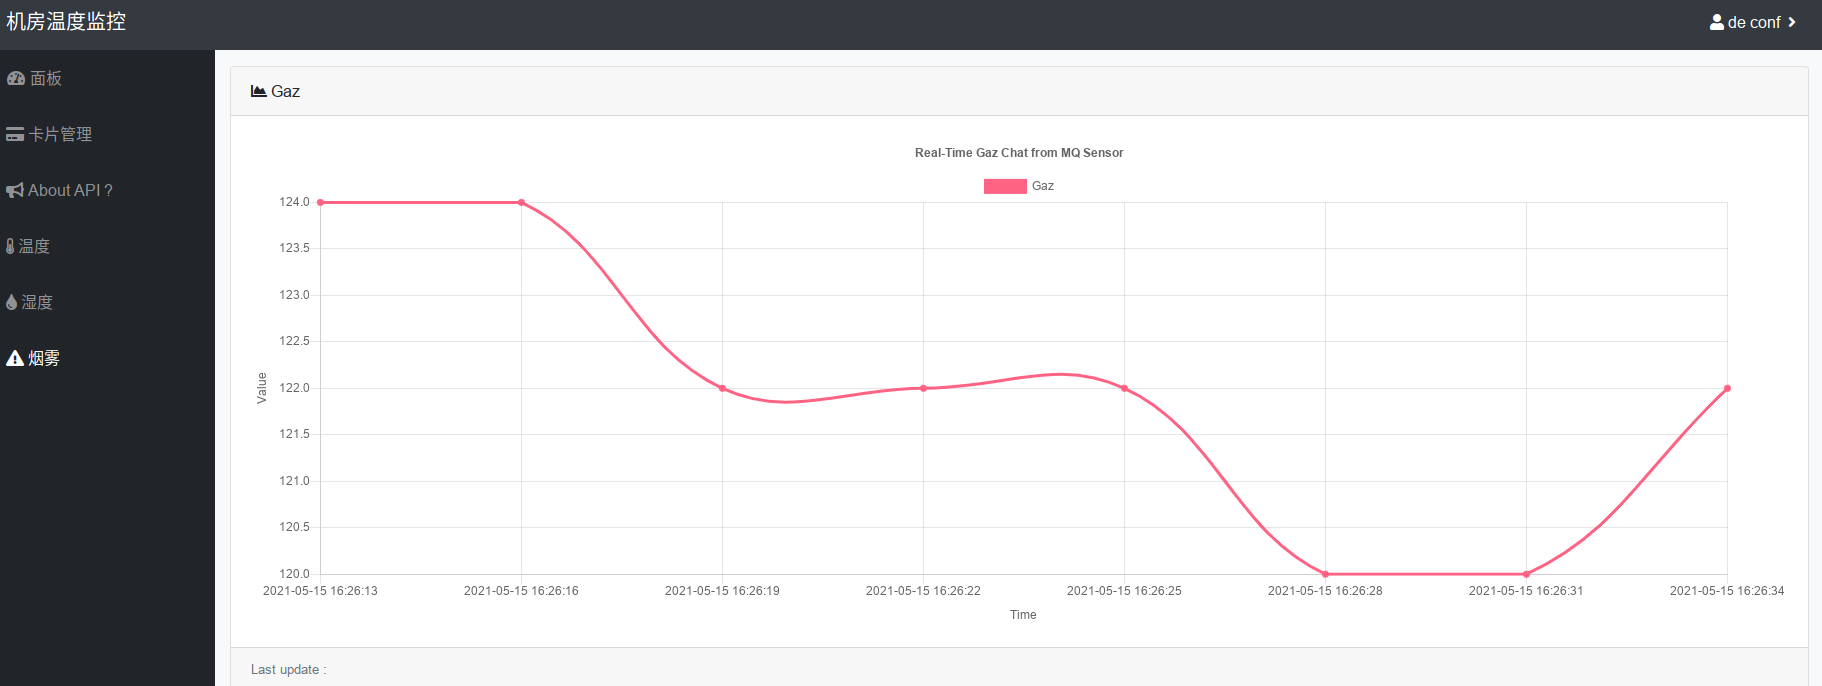
\includegraphics[width=0.85\linewidth]{figure/Gaz}
	\caption{烟雾显示模块}
\end{figure}

\subsubsection{节点管理模块}
通过这里可以方便快捷的对整个节点进行创建,删除。以及节点接受到数据的次数统计。通过次数统计可以对于客户端的传感器有鉴别,防止传感器因接线不良,传感器损坏导致的数据无法传输的问题。以及直观看到节点的API扩展信息。预留了数据整合的基础。
\begin{figure}[H]
	\centering
	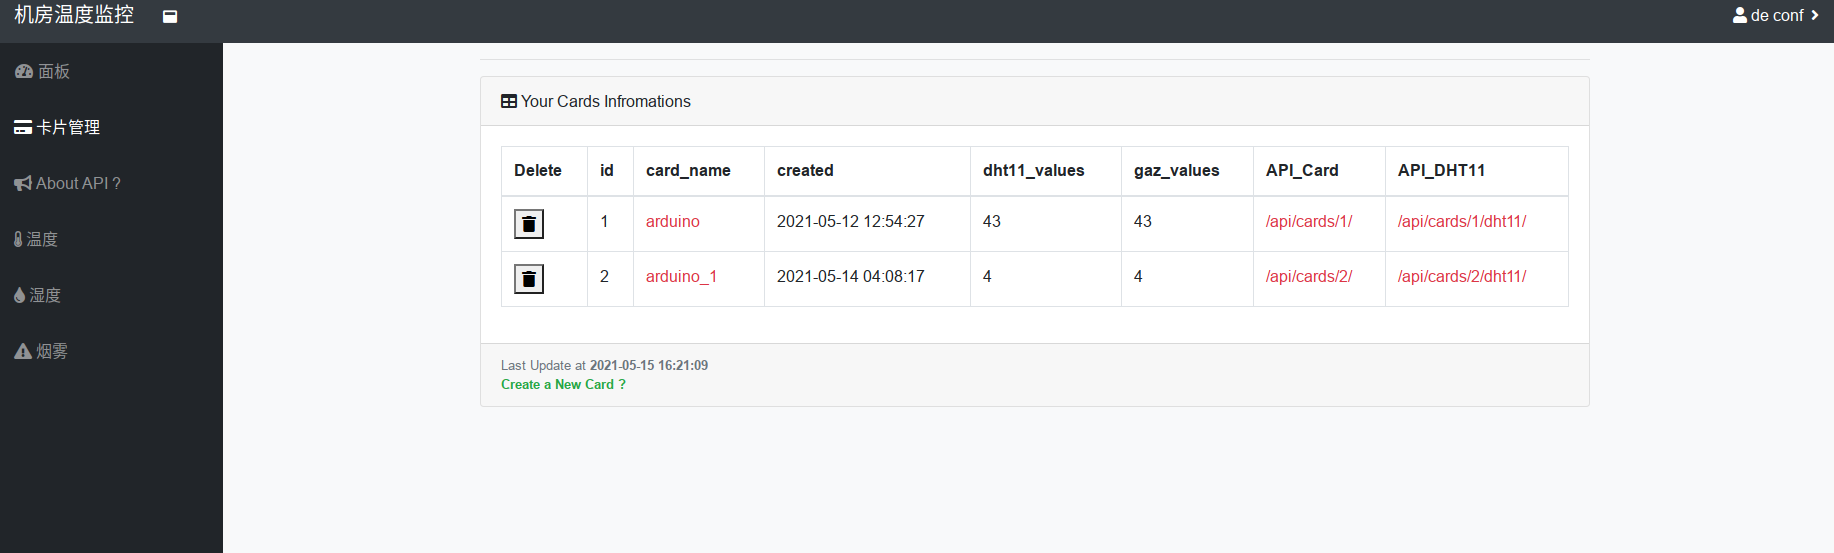
\includegraphics[width=0.85\linewidth]{figure/cards_edit}
	\caption{用户节点管理模块}
\end{figure}
\begin{figure}[H]
	\centering
	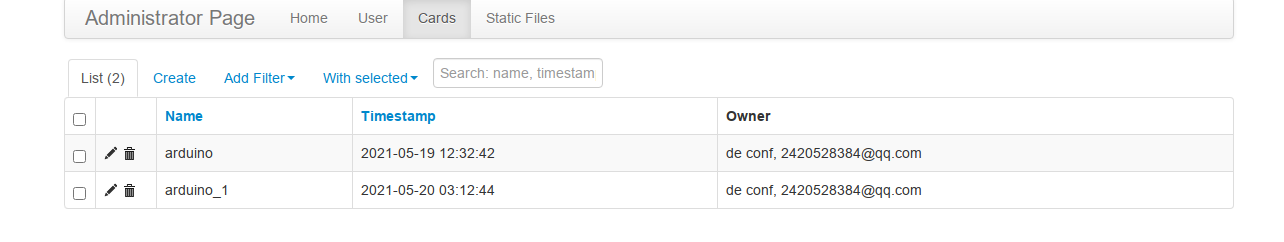
\includegraphics[width=0.85\linewidth]{figure/card_manage}
	\caption{管理员节点管理模块}
\end{figure}

\subsection{Arduino 客户端}

Arduino客户端主要负责节点环境信息采集,以及根据环境信息,控制空调。在各个传感器模块组装以及程序写入之后完成客户端的各项能力。通过DHT11温湿度传感器实现了环境温度、湿度信息采集,MQ2烟雾传感器模块实现了环境烟雾监测,并通过扩展的W5100以太网扩展模块向服务器传输节点的各项信息,如:温度,湿度,烟雾等环境信息。红外接收模块可以进行空调遥控器红外编码的解析,之后将解析后的数据保存在开发板内,可以通过开发板的红外发射模块,依照环境条件的阈值,进行相应的温湿度控制。

Arduino客户端的高扩展性和以及高开放性的特性在本次系统的起到了关键性作用。高扩展体现在Arduoino支持的多传感器设备,高开放性体现在代码中有各类对开源代码的复用。其设备的便捷性和可开发等特性带来了灵活便捷的组装或改装方式。例如,针对与WIFI联网环境可以替换W5100以太网模块为ESP8266模块即可完成WIFI下网络数据传输。在这些特性的支持下,Arduino的客户端具有了便捷的数据采集,传输方式。 

\begin{figure}[htbp]
	\centering
	\includegraphics[width=15cm, height=9cm]{figure/5-10}
	\caption{Arduino客户端展示图}
\end{figure}

\newpage
\subsection{遇到的问题和解决办法}
1. Arduino程序中断。具体表现为:只有串口连接后,程序才继续执行。
\\解决办法: 

阅读官方文档可知从Arduino IDE 1.0开始,串行传输是异步的。如果发送缓冲区中有足够的空白空间,Serial.write()则将在串行传输任何字符之前返回。如果发送缓冲区已满,Serial.write()则将阻塞直到缓冲区中有足够的空间。因此,为避免阻塞调用Serial.write(),需要注释掉程序中调试部分Serial.print()函数,防止引起IO阻塞。

2. Arduino开发板容量有限,无法存储空调设备的全部编码信息。
\\解决办法:

目前临时采用减少空调编码使用,减少空调的控制预设。在后期的优化中设想空调全部编码信息全部存储在服务器数据库中,之后通过MQTT协议进行下发,在通过数据拼接形成完整编码。

3. 红外发射后无反馈机制导致无法判定红外发射后空调是否相应以及生效。
\\解决办法:

通过增加声音感应模块确认空调接受的提示音。从而判断是否接受到Arduino红外控制信号。
